\chapter{Orchestrating Transformation Networks 
    \pgsize{20 p.}
}
\label{chap:orchestration}

\todo{Beispiel warum mehrfache Ausführung nötig, warum also manche Infos erst durch andere bx reinkommen, die bei einer bx isoliert nicht relevant sind.}

\todo{Zeigen: ionfluenz führt zu Konvergenz. Aber konfluenz ist zu s arke Anforderung, außerdem heißt Konvergenz, dass egal welche Reihenfolge der Transformationen man wählt am Ende immer das gleiche Ergebnis rauskommt. Das muss aber nicht so sein. Gebe Beispiel mit groß klein Schreibung, wo je nach Reihe folge verschieden elosungen rauskommen}

\todo{Diss: Konvergenz einführen, hinreichende Eigenschaft? Notwendige Eigenschaft?}

\todo{Property for orchestration: if no consistent solution found then there is no further transformation that could be executed without alternation or because no transforamtion is applicable (undefined for current state, e.g. because of monotony)}


Zu diskutierende Dinge:
\begin{itemize}
    \item Im Allgemeinen könnte eine Transformation beliebige dieser Deltasequenzen modifizieren. Wir verlangen jedoch, dass eine Transformation nur Deltas anhängt, also die Sequenzen länger werden
    \item Genauer beschränken wir auch, welche Sequenzen eine Transformation sehen und ändern darf, genau gesagt darf sie die Sequenzen von zwei Modellen sehen und eine davon verlängern.
    \item Hier kommt bereits der Unterschied zu bisherigen Transformationen, denn die sehen nur Deltas an einem Modell und erzeugen Deltas an dem anderen. Das ist bei uns schon gänzlich anders. Bidirektionale Transformationen unterstützen das im Übrigen auch nicht, sondern sind nur Spezifikationen, aus denen sich Wiederherstellungsroutinen für beide Richtungen ableiten lassen (siehe Stevens 2010)
\end{itemize}


Trivialisierung des Problems:
\begin{itemize}
    \item Ohne weitere Annahmen ist das immer dadurch erreichbar, dass die Transformationen einen beliebigen anderen Zustand der Modelle produzieren. Im einfachsten Fall liefert jede Transformation immer die gleichen konsistenten Modelle zurück, unabhängig von der Änderung. Dann ist der Endzustand der Modelle nach der Ausführung des Netzwerks immer der gleiche.
    \item Das ist im allgemeinen aber nicht Fall. Letztendlich trifft jede Transformation lokale Entscheidungen. Beispielsweise könnte jede einzelne Transformation gegeben eine beliebige Änderung immer dieselben Modelle (bzw. Änderungen die dazu führen) zurückliefern (im trivialsten Fall leere Modelle). Dann erfüllt jede Transformation ihre Korrektheitseigenschaft bzgl. ihrer Relation, aber das Netzwerk muss nicht korrekt sein, da bspw. T(A,B) und T(B,C) sich immer für verschiedene Instanzen von B entscheiden. Es gäbe somit nie eine konsistente Lösung für eine beliebige Ausführungsreihenfolge der Transformationen, auch wenn die Relationen das erlauben würden.
    \item Beispiel mit Namen, wo eine Transformation immer den großen Namen zurückliefert, die andere immer den kleinen. T(A,B) bildet A auf gleiches B ab und beide auf kleine Schreibweise, obwohl beide erlaubt sind. Erzeuge A="a", dadurch B="a". T(B,C) bildet B auf C ab und beide auf große Schreibweise, obwohl beide erlaubt sind. Somit macht sie das zu B="A" und C="A". Nun wird T(A,B) wieder beide klein machen usw. Allerdings wäre eine insgesamt valide Lösung einfach alle groß oder alle klein zu machen, aber die Transformationen finden diesen Zustand nicht. 
    \item Allgemeiner ist zu sagen, dass ein Transformationsnetzwerk eine Turing-Maschine emulieren kann. \todo{Nachweisen!}
    Im allgemeinen terminiert das Netzwerk somit nicht, schlimmer noch, es ist unentscheidbar, ob das Netzwerk hält (siehe Halteproblem).
    \item Dies zeigt bereits, dass keine Ausführungsfunktion definiert werden kann, die immer ein konsistentes Ergebnis liefert.
    \item Wir versuchen daher Annahmen an Transformationen zu finden, um diese Fälle auszuschließen bzw. systematisch zu verringern. 
    \item Außerdem möchten wir eine Ausführungsfunktion haben, die ein konsistentes Ergebnis liefert oder einen Fehler, denn es muss nicht immer eine korrekte Lösung geben. Ziel ist es dann die Anzahl der Fälle, in denen sie einen Fehler zurückgibt, zu reduzieren.
\end{itemize}


Zielsetzung:
\begin{itemize}
    \item Korrekte Anwendungsfunktion finden (in bestehenden Arbeiten~\cite{stevens2017a}) auch "Resolution" genannt (formal definieren!):
    \item Welche Anforderungen müssen wir dafür an die Transformationen stellen, damit solch eine Funktion definiert werden kann?
    \item Wir bezeichnen das Transformationsnetzwerk, in dem eine Transformation eingesetzt wird, als "Kontext"
    \item Welche dieser Eigenschaften kann die einzelne Transformation (ohne Kenntnis der anderen) erfüllen und für welche muss der Kontext (d.h. die anderen Transformationen) bekannt sein?
    \item $\Rightarrow$ Interesse an "kontextfreien" Eigenschaften (lassen sich ohne Kenntnis der anderen Transformationen sicherstellen -> Wiederverwendbarkeit) und "kontextsensitiven" Eigenschaften (Erfüllung der Eigenschaft nur durch Kenntnis über das Transformationsnetzwerk möglich)
    \item Kontextfreie Eigenschaften involvieren solche, die wir eh schon von Transformationen kennen (Korrektheit einer Transformation, Hippokratie etc.) und solche, die dadurch zustande kommen, dass man weiß, dass diese Transformation in einem Netzwerk eingesetzt werden soll.
    \item Zielsetzungsoptionen:
    \begin{itemize}
        \item Wir schränken die Transformationen so ein, dass es immer mindestens eine Ausführungsreihenfolge der Transformationen gibt, sodass für jede beliebige Änderung ein konsistentes Ergebnis durch Anwenden der Transformationen gefunden werden kann
        \item Wir akzeptieren, dass es Änderungen gibt, für die das Netzwerk kein konsistentes Ergebnis produzieren kann. Dann muss das Netzwerk (mindestens) in diesen Fällen mit einer Fehlermeldung terminieren.
        \item Eine Option ist, dass das Netzwerk dieses Verhalten nur approximiert bzw. approximieren kann, dann muss es sich konservativ verhalten, d.h. im Fall, dass es keine Lösung gibt, auf jeden Fall eine Fehlermeldung geben, und im Fall, in dem es eine Lösung gibt, diese bestenfalls finden oder ausgeben, dass es keine finden kann (d.h. keine False Positives bzw. Nicht-Terminierung). Ziel ist es dann den Grad der Konservativität zu minimieren.
    \end{itemize}
    \item Lösungsoptionen (Grad der Einschränkung an die Transformationen):
    \begin{itemize}
        \item Hohe Einschränkung: Jede beliebige Reihenfolge von ausgeführten Transformationen führt letztendlich zu einem korrekten Ergebnis (Fixpunktiteration -- Allquantifizierung) -- Hippokratie-Eigenschaft sorgt dafür, dass keine Transformation wieder etwas ändert, wenn Konsistenz bereits hergestellt ist.
        Diese Eigenschaft ist in der Praxis möglicherweise zu strikt, da sie sehr starke Anforderungen an die Transformationen stellen müsste. Dafür wäre aber die Anwendungsfunktion trivial.
        \item Mittlere Einschränkung: Es gibt eine Reihenfolge von ausgeführten Transformationen für jede Änderung die terminiert (Existenzquantifizierung) und die Ausführungsfunktion findet diese Reihenfolge.
        Utopisch, dass die Anwendungsfunktion aus (potentiell sehr mächtigen) Transformationen die richtige Reihenfolge errechnen kann. Dafür aber (möglicherweise) weniger Anforderungen an die Transformationen (zumindest nicht mehr Anforderungen, denn die Allquantifzierung induziert die Existenzquantifizierung). Eine Funktion könnte dann zumindest nach best-effort versuchen, die richtige Reihenfolge zu finden und konservativ abbrechen, wenn sie diese nicht finden kann (also entweder konsistent terminieren oder terminieren mit der Aussage, dass es entweder keine solche Reihenfolge gibt -- bei relaxierten Anforderungen -- oder dass es sie nicht finden kann).  
        \item Geringe Einschränkung: Es gibt potentiell keine Reihenfolge der Transformationen, die bei einer Änderung zu einer konsistenten Lösung kommt. Hier müsste die Ausführungsfunktion entsprechend einen Fehler ausgeben.
        \item Bestehende Arbeiten (\cite{stevens2017a}) schlagen auch vor eine Baumstruktur zu berechnen (Spannbaum), in dem nur entlang der Baumkanten die Transformationen ausgeführt werden. Dies ist jedoch eine starke Einschränkung daran, was die Transformationen ausdrücken können. Betrachtet man beispielsweise PCM, UML und Java, und hat eine Änderung in PCM. Dann könnte der Spannbaum entweder PCM -> UML -> Java sein, oder PCM -> UML + PCM -> Java. In ersterem Fall würde Verhaltensbeschreibung, die von PCM nach Java übertragen, aber in UML nicht dargestellt wird, nicht übertragen. Im zweiten Fall würde zusätzliche Information zwischen UML und Java nicht propagiert (Beispiel?) --> Hier sollte auf das Properties-Kapitel verwiesen werden, wo diese "Bottlenecks" erklärt sein sollten, inklusive einem Beispiel, die allgemein Baumstrukturen für Transformationsnetwerke ausschließen.
    \end{itemize}
    \item Dies setzt voraus, dass die Transformationen und die Anwendungsfunktion mit jeder beliebigen Nutzer-Änderung umgehen kann. Man kann jedoch auch verlangen, dass die Anwendungsfunktion genau dann, wenn es überhaupt eine Ausführungsreihenfolge gibt, diese findet, und sonst einen Fehler ausgibt.
    \item \textbf{Wichtig:} Im Allgemeinen kann eine Ausführungsfunktion keine terminierende Reihenfolge berechnen, da die Transformationen Turing-vollständig sind und deshalb die Frage, welche Reihenfolge zu einer Terminierung führt, unentscheidbar ist (Halteproblem). Daher können wir nur einen konservativen Algorithmus angeben, der ein sinnvolles Abbruchkriterium definiert, mit dem die Ausführung beendet wird, auch wenn potentiell eine Lösung hätte gefunden werden können. Die Fragestellung ist also, wie die Ausführungsfunktion aussehen muss, damit sie in möglichst vielen Fällen, in denen es eine terminierenden Reihenfolge gibt, diese auch findet. Insbesondere lässt sich somit keine geschlossene Form für die Ausführungsfunktion angeben, sondern nur ein Algorithmus, der zur Laufzeit eine Reihenfolge (dynamisch) festlegt.
\end{itemize}


Problemraum:
\begin{itemize}
    \item Ziel ist, dass ein Netzwerk von Transformationen nach einer Änderung in einem konsistenten Zustand terminiert. D.h. Korrektheit stellt Anforderungen an \emph{Terminierung}, sowie den \emph{Zustand} bei Terminierung.
    \item Folgende Abweichungen davon können auftreten:
    \begin{enumerate}
        \item Nicht-Terminierung: Das Netzwerk terminiert nicht. Das bedeutet im Prinzip, dass die Ausführungsfunktion (bzw. der Laufzeit-Algorithmus, der die Funktion dynamisch emuliert) nicht \emph{sound} ist. Soundness der Ausführungsfunktion setzt voraus, dass die berechnet Aufrufsequenz endlich ist. Wenn die Ausführung nicht terminiert, bedeutet das, dass entweder die gleichen Zustände mehrfach durchlaufen werden oder eine Sequenz unendlich vieler Zustände produziert wird. Denn wenn beides nicht der Fall ist, gibt es eine endliche Sequenz unterschiedlicher Zustände, d.h. Terminierung. Das bedeutet, dass es folgende zwei Möglichkeiten gibt:
        \begin{itemize}
            \item Alternierung: Die gleichen Zustände werden mehrfach durchlaufen.
            \item Divergenz: Es werden unendlich viele Zustände produziert.
        \end{itemize}
        \item Inkonsistente Terminierung: Die Ausführungsfunktion bzw. der Algorithmus beendet die Ausführung, aber in einem inkonsistenten Zustand. Hier lassen sich ebenfalls wieder zwei Fälle unterscheiden.
        \begin{itemize}
            \item Unerkannte Inkonsistenz: Der Algorithmus terminiert und denkt, der Zielzustand wäre konsistent. Dies bedeutet aber direkt, dass nicht alle Konsistenzrelationen erfüllt sind, was, zumindest in der Theorie, einfach zu prüfen wäre (entweder durch Prüfung der Relationen oder durch Ausführung der hippokratischen Transformationen, die alle nichts tun dürften)
            \item Erkannte Inkonsistenz: Der Algorithmus terminiert, wissend dass die Lösung nicht konsistent ist. Dies kann entweder sein, weil eine Transformation für zwei Modelle in einem inkonsistenten Zustand nicht mehr anwendbar ist, oder weil irgendein anderes Abbruchkriterium erreicht ist.
        \end{itemize}
    \end{enumerate}
\end{itemize}


Notwendigkeit Transformationen oder Anwendungsfunktion einzuschränken:
\begin{itemize}
    \item Zeigen, dass es Beispiele gibt, in denen es keine einzige Ausführungsreihenfolge gibt (All-Quantifizierung), die zu einem konsistenten Ergebnis führt:
    \item Zeigen, dass es Beispiele gibt, in denen es unabhängig von der Ausführungsreihenfolge immer zu einer Alternierung kommt
    \item Zeigen, dass es Beispiele gibt, in denen es unabhängig von der Ausführungsreihenfolge immer zu einer Divergenz kommt.
    \item Die Beispiele sollten zeigen, dass wir keine Einschränkungen an die Transformationen machen können, was das Problem aushebelt. D.h. egal welche Einschränkungen ich an die Transformationen definiere, es lassen sich immer Beispiele konstruieren, in denen es keine Ausführungsreihenfolge gibt, in denen sie terminieren.
    \item Mathematisch zeigen, dass Alternierung und Divergenz die einzigen Probleme sind. D.h. wenn nicht der gleiche Zustand mehrmals durchlaufen wird (Alternierung) und es nicht unendlich viele Zustände gibt (Divergenz), dann ist die Folge endlich.
    \item Außerdem mathematisch die Abbildung von Transformationen auf Turing-Maschinen zeigen und damit ableiten, dass allgemeine Netzwerke erstmal nicht terminieren müssen (Abbildung auf Halteproblem)
\end{itemize}

Zielsetzung die Zweite:
\begin{itemize}
    \item Wir definieren möglichst minimale Beschränkungen, die dazu führen, dass das Netzwerk terminiert. D.h. es terminiert entweder konsistent oder es terminiert mit einem Fehler, der sagt, dass entweder keine Konsistenz hergestellt werden kann (es gibt keine Ausführungsreihenfolge der Transformationen, die zu Konsistenz führt) oder dass die Anwendungsfunktion nicht in der Lage war eine passende Ausführungsreihenfolge zu finden (Konservativität)
    \item Zwei Arten von Beschränkungen
    \begin{itemize}
        \item Beschränkungen an die Transformationen, die dazu führen, dass es in mehr Fällen mindestens eine Ausführungsreihenfolge gibt, in der das Netzwerk konsistent terminiert
        \item Beschränkungen an die Ausführungsfunktion, sodass die Ausführung auf jeden Fall terminiert, wenn auch konservativ, d.h. mit Fehler, obwohl es eine korrekte Lösung gegeben hätte.
    \end{itemize}
\end{itemize}



Exkurs: Menge (konsistenter) Modelle bildet keinen topologischen Raum
\begin{itemize}
    \item Topologischer Raum besteht aus Grundmenge und Mengensystem von Teilmengen mit den Eigenschaften, dass die Grundmenge offen ist, der Schnitt endlich vieler Mengen offen und die Vereinigung beliebig vieler Mengen offen ist. 
    \item Die Grundmenge wäre die Menge aller Modellelemente
    \item Diese Menge ist normalweise offen, da z.B. für ein Element mit einem String-Attributwert immer noch das Element mit dem gleichen String-Attributwert plus einem weiteren Symbol in der Menge liegt (und man die Ordnung in der Menge entsprechend definiert). Dass ein Metamodell möglicherweise Einschränkungen definiert und dann im schlimmsten Fall nur ein einziges Modell valide ist, lassen wir hier außen vor.
    \item Betrachten wir nun eine Topologie auf dieser Menge, also ein Mengensystem aus konsistenten Modellen. Leider ist jedoch der Schnitt zweier konsistenter Modelle nicht zwangsläufig konsistent. Insbesondere sind diese Mengen auch nicht offen, da sie die abgeschlossene Menge darstellen, die genau ein Modell beschreiben. 
    \item Somit lässt sich die Definition von Topologien hier nicht anwenden.
\end{itemize}



\section{No Execution Order with Consistent Result}

It is obvious that we can define consistency preservation rules for which the orchestration function cannot find an execution order that returns a consistent tuple of models after certain changes. Consider the example in \autoref{fig:formal:noexecutionorder}. There exists no execution order for any input value that terminates. The transformations will always increase the value, although the defined relations could be fulfilled for the input value, but the transformations never find that solution.

\begin{figure}
    \centering
    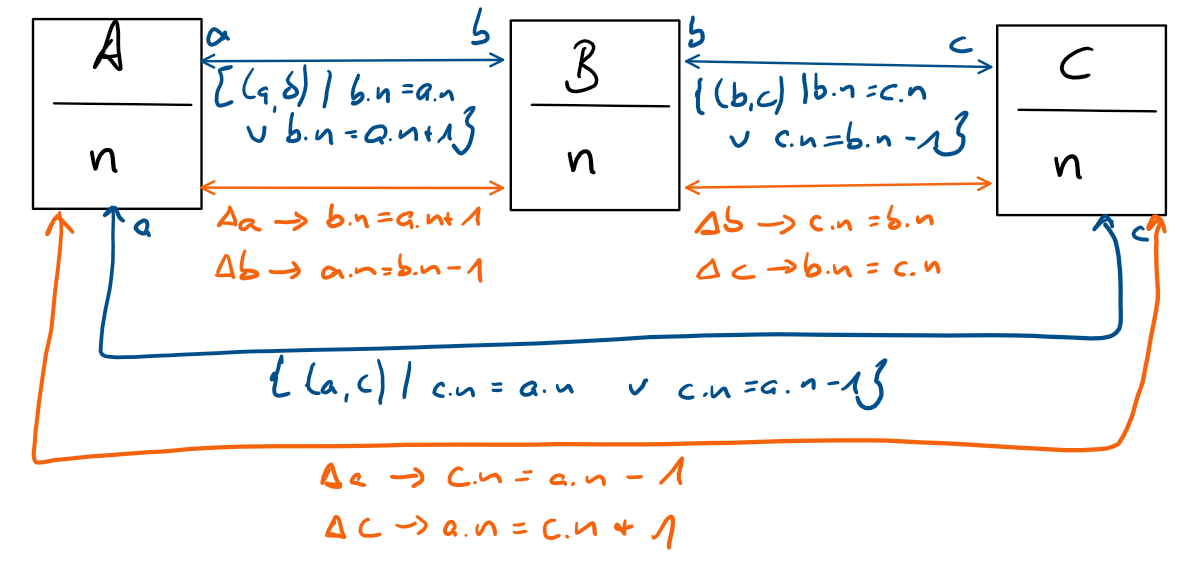
\includegraphics[width=\textwidth]{figures/correctness/formal/divergence_example.png}
    \caption{Example for divergence}
    \label{fig:formal:noexecutionorder}
\end{figure}

Although we will discuss restrictions to relations and transformations that reduce the chance that no solution can be found, it will not be possible to ensure that such a solution can always be found. This is due to the reason that transformations can perform arbitrary changes given that transformations are Turing complete, which should not be restricted, because it is unclear which restrictions could be made without forbidding scenarios that should actually we supported. Thus, we assume that transformations are Turing complete.

We explicitly allow the orchestration function to return a sequence that will, if applied to models and changes to them, not deliver a consistent tuple of models. As discusses, this is supposed to reflect cases in which no such sequence can be calculated.
However, it may be useful to have some notion of \emph{optimality} that ensures that if a sequence that delivers a consistent result exists, the orchestration function is supposed to find it.
Formally, this notion looks as follows.

\begin{definition}[Optimal Consistency Preservation Orchestration Function]
    Let $\consistencypreservationruleset{}$ be a set of consistency preservation rules for a set of consistency relations $\consistencyrelationset{CR}$ on metamodels $\metamodeltuple{M} = \tupled{\metamodelsequence{M}{n}}$.
    We say that an orchestration function $\consistencyorcfunction{\consistencypreservationruleset{}}$ for these rules is \emph{optimal} if it always returns a sequence that delivers a consistent set of models if possible, i.e.,
    \begin{align*}
        &
        \forall \modeltuple{m} \in \metamodeltupleinstanceset{M} : \forall \changetuple{\metamodeltuple{M}} = \tupled{\change{\metamodel{M}{1}}, \dots, \change{\metamodel{M}{n}}} \in \changeuniverse{\metamodeltuple{M}} :
        \modeltuple{m} \consistenttomath \consistencyrelationset{CR} \Rightarrow \\
        & \formulaskip
        \bigl[ \bigl(
            \exists \consistencypreservationrule{1}, \dots, \consistencypreservationrule{m} \in \consistencypreservationruleset{} : 
            \exists \changetuple{\metamodeltuple{M}}' = \tupled{\change{\metamodel{M}{1}}', \dots, \change{\metamodel{M}{n}}'} \in \changeuniverse{\metamodeltuple{M}} :\\
            & \formulaskip \formulaskip
            \cprgeneralizationfunction{\consistencypreservationrule{1}} \concatfunction \dots \concatfunction \cprgeneralizationfunction{\consistencypreservationrule{m}}(\modeltuple{m}, \changetuple{\metamodeltuple{M}}) = (\modeltuple{m}, \changetuple{\metamodeltuple{M}}')\\
            & \formulaskip \formulaskip
            \land \tupled{\change{\metamodel{M}{1}}'(\model{m}{1}), \dots, \change{\metamodel{M}{n}}'(\model{m}{n})} \consistenttomath \consistencyrelationset{CR} \bigr) \\
            & \formulaskip
            \Rightarrow \bigl(        
            \exists \consistencypreservationrule{1}', \dots, \consistencypreservationrule{m}' \in \consistencypreservationruleset{} : 
            \exists \changetuple{\metamodeltuple{M}}'' = \tupled{\change{\metamodel{M}{1}}'', \dots, \change{\metamodel{M}{n}}''} \in \changeuniverse{\metamodeltuple{M}} :\\
            & \formulaskip \formulaskip
            \consistencyorcfunction{\consistencypreservationruleset{}}(\modeltuple{m}, \changetuple{\metamodeltuple{M}}) = \tupled{\consistencypreservationrule{1}', \dots, \consistencypreservationrule{m}'} \\
            & \formulaskip \formulaskip
            \land \cprgeneralizationfunction{\consistencypreservationrule{1}'} \concatfunction \dots \concatfunction \cprgeneralizationfunction{\consistencypreservationrule{m}'}(\modeltuple{m}, \changetuple{\metamodeltuple{M}}) = (\modeltuple{m}, \changetuple{\metamodeltuple{M}}'')\\
            & \formulaskip \formulaskip
            \land \tupled{\change{\metamodel{M}{1}}''(\model{m}{1}), \dots, \change{\metamodel{M}{n}}''(\model{m}{n})} \consistenttomath \consistencyrelationset{CR}
        \bigr) \bigr]
    \end{align*}
\end{definition}

Unfortunately, optimality is a property that we cannot request from an orchestration function. Optimality would mean that the orchestration function can decide whether there is sequence of transformations that leads to consistent models and thus terminate.
Due to Turing-completeness of the network this would mean that the orchestration function can decide whether a Turing machine halts, which is proven impossible.
Thus, our only goal can be to achieve optimality as far as possible in terms of reducing the degree of conservativeness, i.e., reduce the cases in which no sequence is found although it exists.

We can define a measure for the optimality of an orchestration function:
\begin{align*}
    &
    Optimality_{\consistencyorcfunction{\consistencypreservationruleset{}}} = \frac{\mathtext{\# of model / delta pairs for which the function finds an order that terminate consistently}}{\mathtext{\# of model / delta pairs for which an order that terminates consistently exists}}
\end{align*}

In fact, both these numbers usually infinite, an there is an infinite number of possible models and deltas. However, it does finally not matter for us what the actually value is, but only how to improve that value.
\todo{We have to map that value to compatibility, which reduces the number of potential false orders.}
